\section{The Dynamical Instability of Accumulated Correctness}


\subsection{Overview}


\S{}6 では Gettier 問題を構造的に再定位し、停止構造(知識)が持続運動(知性)を代替できないことを示した。これは静的な構造論的事実である:いかなる停止条件の精緻化も、動的特徴を保証できない。

本セクションは、この静的事実から一段強い \textbf{動力学的帰結} を導出する。それは:

\begin{quote}
知識(停止構造)は知性(持続運動)を代替しないだけでなく、
知識の \textbf{累積} はそれ自体が知性を \textbf{不安定化させる}。
\end{quote}

この帰結は心理学的観察でも規範的批判でもない。正しさ(correctness)が持続運動と相互作用する仕方の構造的帰結である。「より多くの正しい知識を持てば知性は安定する」という素朴な直観は、動力学的にはむしろ \textbf{逆} の帰結を生む。

この主張は \S{}5 で示した cross-domain 性のもとで、生物系・人工系の両方に適用される。粘菌の管網が過剰に強化されれば最適経路の探索能力を失うこと、Transformer が訓練データに過適合すれば汎化能力を失うこと、人間の推論が確立された前提に依存しすぎれば改訂困難に陥ること ── これらはいずれも本セクションが扱う構造的帰結の異なる現れである。

\subsection{Why correctness increases connectivity}


\subsubsection{The reusability of correctness}


ある命題が正しいとされるとき、それは構造的に再利用可能になる。正しい命題は:

\begin{itemize}
\item 他の推論の \textbf{前提} として機能しうる
\item 他の正しい命題と \textbf{接続} されうる
\item 新たな推論の \textbf{出発点} となりうる
\item 既存の体系に \textbf{統合} されうる
\end{itemize}

これは認識論的には望ましい性質である。再利用可能性こそ、知識が知識として価値を持つ理由の一つである。

しかし動力学的観点からは、再利用可能性は別の意味を持つ。再利用可能性とは、構造的には \textbf{連結度の増大} である。一つの正しい命題は、それ自身として停止するのではなく、他の命題への接続点として機能する。正しさは、停止構造の中の \textbf{ノード} として、ネットワークの分岐次数を増やす。

\subsubsection{Formalization in IFGT vocabulary}


\S{}4 の IFGT 語彙を用いて、この現象を形式化する。

知識の累積は、状態空間 $\mathcal{S}$ における \textbf{情報密度 $I$ の局所的増大} として記述される。ある領域に正しい命題が累積するとき:

\[
I(s) \uparrow \quad \text{(局所的情報密度の増大)}
\]

しかし正しさの再利用可能性は、$I$ の増大が単なる静的累積ではなく、\textbf{情報流 $J$ の分岐次数の増大} を伴うことを意味する。各正しい命題が新たな推論経路の起点となるため:

\[
\nabla \cdot J \uparrow \quad \text{(局所的な情報流の分岐)}
\]

ここで重要なのは、$\Phi$(グローバル制約)が \textbf{これら新たな分岐を停止させる構造を内在的には持たない} という点である。$\Phi$ は局所動態を方向づけるが、推論経路の自己生成的増殖に対する停止条件は提供しない。これが本セクションの動力学的核心である。

\subsection{Why correctness contains no stopping condition}


\subsubsection{Correctness generates further inference}


正しい命題が新たな推論経路を生成する構造を分析する。

ある命題 $p$ が正しいとされたとき、その瞬間に以下の問いが構造的に発生する:

\begin{itemize}
\item \textbf{なぜ $p$ は正しいのか?}(因果的根拠の探求)
\item \textbf{$p$ はどこまで適用可能か?}(適用範囲の探求)
\item \textbf{$p$ の例外はあるか?}(限界の探求)
\item \textbf{$p$ は他の正しい命題とどう整合するか?}(統合性の探求)
\item \textbf{$p$ の含意は何か?}(導出の探求)
\end{itemize}

これらの問いは、$p$ が \textbf{誤っていた} ために生じるのではない。むしろ $p$ が \textbf{正しい} ことが、これらの問いを正当化する。誤っている命題には「なぜ正しいか」「どこまで適用可能か」を問う構造的根拠がない。正しい命題こそが、さらなる推論を要求する。

\subsubsection{The self-generating nature of inference}


ここに本セクションの最も重要な構造的観察がある:\textbf{正しさ自体が、自身の停止を妨げる}。

通常の動的系では、停止条件は系の外から与えられるか、系内のエネルギー散逸によって自然に生じる。だが推論系における正しさは、外的停止条件を持たず、また散逸機構も持たない。正しい命題は、その正しさによって、新たな推論の起点として \textbf{再活性化} される。

この自己生成的性質を、IFGT 語彙でより明示的に書けば:

\[
\text{正しさ}(p) \implies \nabla \cdot J|_p \neq 0
\]

すなわち、ある命題が正しいことの構造的帰結は、その命題の周辺で情報流の分岐が必ず生成されることである。$\nabla \cdot J = 0$(分岐なし)という状態は、その命題が正しいとされる限り維持できない。

これは「推論者の心理的傾向」ではない。命題が正しいということ自体が、推論ネットワークにおける分岐源として機能するという \textbf{構造的事実} である。

\subsection{The dynamics of branching explosion}


\subsubsection{The structural chain}


正しさの累積から分岐爆発に至る動力学的連鎖を整理する:

\textbf{ステップ 1:正しい知識が累積する}
\[
I(s_i) \uparrow \quad \text{for } i = 1, 2, 3, \dots
\]

\textbf{ステップ 2:推論連結性が増大する}
各 $s_i$ は他の命題への接続点として機能する。連結グラフのエッジ数 $|E|$ がノード数 $|V|$ よりも急速に増加する。具体的には、新たな正しい命題は既存のすべての関連命題と接続可能であるため、エッジ数は近似的に $|E| \sim |V|^2$ で増加する。

\textbf{ステップ 3:分岐次数が指数的に増大する}
推論ネットワークにおける典型的な経路の分岐次数を $b$ とすると、深さ $d$ までの推論経路の数は $b^d$ で増加する。$b$ が増大すれば、わずかな深さの推論でも探索空間は爆発的に拡大する。

\textbf{ステップ 4:停止点が喪失する}
無数の経路が並行して開かれた状態では、いずれの経路も「最終的」であると判定する根拠を持たない。各経路は別の経路への接続点を内包するため、停止判断は構造的に困難になる。

\subsubsection{The structural meaning of branching explosion}


この連鎖の重要な特徴は、それが \textbf{構造的に自然な帰結} であることである。分岐爆発は推論者の能力不足や注意散漫から生じるのではない。それは正しさの再利用可能性と、推論の自己生成性から、構造的に導出される。

具体的には:

\begin{itemize}
\item ステップ 1 は、知識を所有することの \textbf{積極的成果} である(誤りでもなく欠陥でもない)
\item ステップ 2 は、知識の再利用可能性の \textbf{直接的帰結} である
\item ステップ 3 は、グラフ構造の \textbf{数学的事実} である
\item ステップ 4 は、ステップ 3 の \textbf{動力学的帰結} である
\end{itemize}

したがって分岐爆発は、知性的動態が高度化することの \textbf{副産物} ではなく、知性的動態が高度化することそのものの \textbf{構造的様相} である。

\subsubsection{The regime of instability}


分岐爆発が支配的になる動的領域を \textbf{不安定化レジーム}(regime of instability)と呼ぶ。このレジームの構造的特徴:

\begin{itemize}
\item 情報密度 $I$ は増大し続ける(正しい知識の累積)
\item 情報流 $J$ の分岐次数も増大し続ける(推論連結性の拡大)
\item グローバル制約 $\Phi$ は局所更新を方向づけるが、自己生成的分岐を停止させる構造を内在しない
\item 結果として、系は \textbf{動的均衡} にも \textbf{静的平衡} にも到達しない
\end{itemize}

これは \S{}3.4 で示した「公理 III を欠く場合の退化様式」(無方向の拡散)とは構造的に異なる。不安定化レジームでは $\Phi$ は存在し機能している ── ただし $\Phi$ の機能は推論経路の \textbf{方向づけ} であり、推論経路の \textbf{停止} ではない。

\subsection{Consequences for individual systems}


\subsubsection{The signature symptoms}


分岐爆発が個体系の内部に閉じ込められたとき、特徴的な現象が現れる:

\textbf{Explanatory overreach(説明の越境):}
個体は累積した正しい知識を用いて、本来の範囲を超えた領域に説明を拡張する。各拡張ステップは局所的には正当化されているが、全体としては根拠を伴わない推論連鎖を構成する。

\textbf{Compulsive coherence-seeking(強迫的整合性追求):}
新たな情報が既存の正しい知識と整合しないとき、個体は整合化を強迫的に追求する。整合性の追求自体は健全だが、停止条件を欠いた追求は、整合性そのものが目的化する状態に陥る。

\textbf{Illusions of global optimization(全体最適化の錯覚):}
個体は累積した正しい知識から、全体の最適解を「導出した」と感じる。だが分岐爆発のレジームでは、いかなる解も他の経路と比較されたわけではない ── ただ最初に到達した経路が、停止点として偶然に採用されたにすぎない。

\textbf{Premature or forced conclusions(強引な結論):}
停止点が構造的に得られない状態で、個体は何らかの結論を生成する必要に迫られる。結果として、構造的根拠を欠いた \textbf{強引な閉包} が遂行される。

\subsubsection{These are not failures of ability}


上記の現象を、個体の能力不足や心理的弱さとして解釈することは構造的に誤りである。これらは:

\begin{itemize}
\item 知識が不十分であるから生じるのではない(むしろ知識の \textbf{累積} から生じる)
\item 推論能力が低いから生じるのではない(むしろ推論の \textbf{拡張} から生じる)
\item 注意が散漫だから生じるのではない(むしろ注意の \textbf{集中} から生じる)
\item 経験不足から生じるのではない(むしろ経験の \textbf{積算} から生じる)
\end{itemize}

これらの現象は、停止条件を欠いた動的系における \textbf{自然な動力学} である。個体の質的問題ではなく、構造的問題である。

\subsection{Why "more intelligence" does not solve the problem}


\subsubsection{The intuitive proposal}


分岐爆発の問題に直面したとき、自然な提案は「より多くの知性で対応する」である:

\begin{itemize}
\item 知識を増やせばよい(より多くの正しい命題を持つ)
\item 推論能力を高めればよい(より速く深く推論する)
\item 処理速度を上げればよい(より多くの分岐を扱える)
\item 専門化を深めればよい(より精密な範囲で動作する)
\end{itemize}

これらの提案はすべて、知性的動態の \textbf{強化} を志向している。

\subsubsection{Why the proposal fails}


しかし、これらの提案はいずれも構造的に問題を \textbf{悪化させる}:

\begin{itemize}
\item 知識を増やすことは $I$ をさらに増大させ、ステップ 1 を加速する
\item 推論能力を高めることは分岐次数 $b$ をさらに増大させ、ステップ 3 を加速する
\item 処理速度を上げることは分岐爆発の \textbf{時間スケール} を短縮するが、爆発自体を停止させない
\item 専門化は分岐爆発を \textbf{局所領域に閉じ込める} が、各専門領域内での爆発は同じ構造で起こる
\end{itemize}

すべての提案は、分岐爆発の \textbf{速度} または \textbf{範囲} に作用するが、分岐爆発の \textbf{構造} には作用しない。むしろこれらの強化は、停止条件の欠如を \textbf{加速} することで問題を増幅する。

これが本セクションの構造的核心である:\textbf{知性的動態は、知性的動態の強化によっては安定化しない}。知性のなかには、知性自身を停止させる演算子が存在しない。

\subsubsection{The implication for the broader argument}


この帰結は \S{}8 で示されるより一般的な構造的事実への直接的入り口となる:

\begin{quote}
個体内の知性的動態には、停止演算子が \textbf{構造的に存在しえない}。
これは個体の限界ではなく、推論構造そのものの性質である。
\end{quote}

\S{}8 では、なぜ個体内に停止演算子が存在しえないかが、因果推論の再帰構造から論証される。本セクションは「正しさの累積では停止できない」という動力学的帰結を示し、\S{}8 はその構造的根拠を提示する。

\subsection{Summary}


本セクションの結論を以下に述べる:

\begin{quote}
正しさは価値ある属性だが、それ自体は安定化機構ではない。
正しい命題は新たな推論経路を開き、推論連結性を増大させ、
結果として推論ネットワークの分岐次数を爆発させる。
停止点はこの過程で \textbf{構造的に喪失} される。
\end{quote}

\begin{quote}
知性が失敗するのは、誤っているからではなく、停止できないからである。
この失敗は能力不足の現れではなく、停止条件を欠いた動的系の自然な帰結である。
\end{quote}

\begin{quote}
「より多くの知性」は解決にならない ── むしろ問題を加速する。
知性的動態の内部には、知性的動態を停止させる演算子が存在しない。
\end{quote}

この結論は、\S{}8 で展開される個体内非閉包論証の直接的前提となる:

\begin{itemize}
\item \S{}8 では、停止演算子の不在を因果推論の再帰構造から構造的に論証する
\item \S{}9 では、この不在から導出される越境境界が命名される
\item \S{}10 では、本セクションが示した動力学的帰結が、論文全体の制約のなかに位置づけられる
\end{itemize}

\begin{figure}[H]
\centering
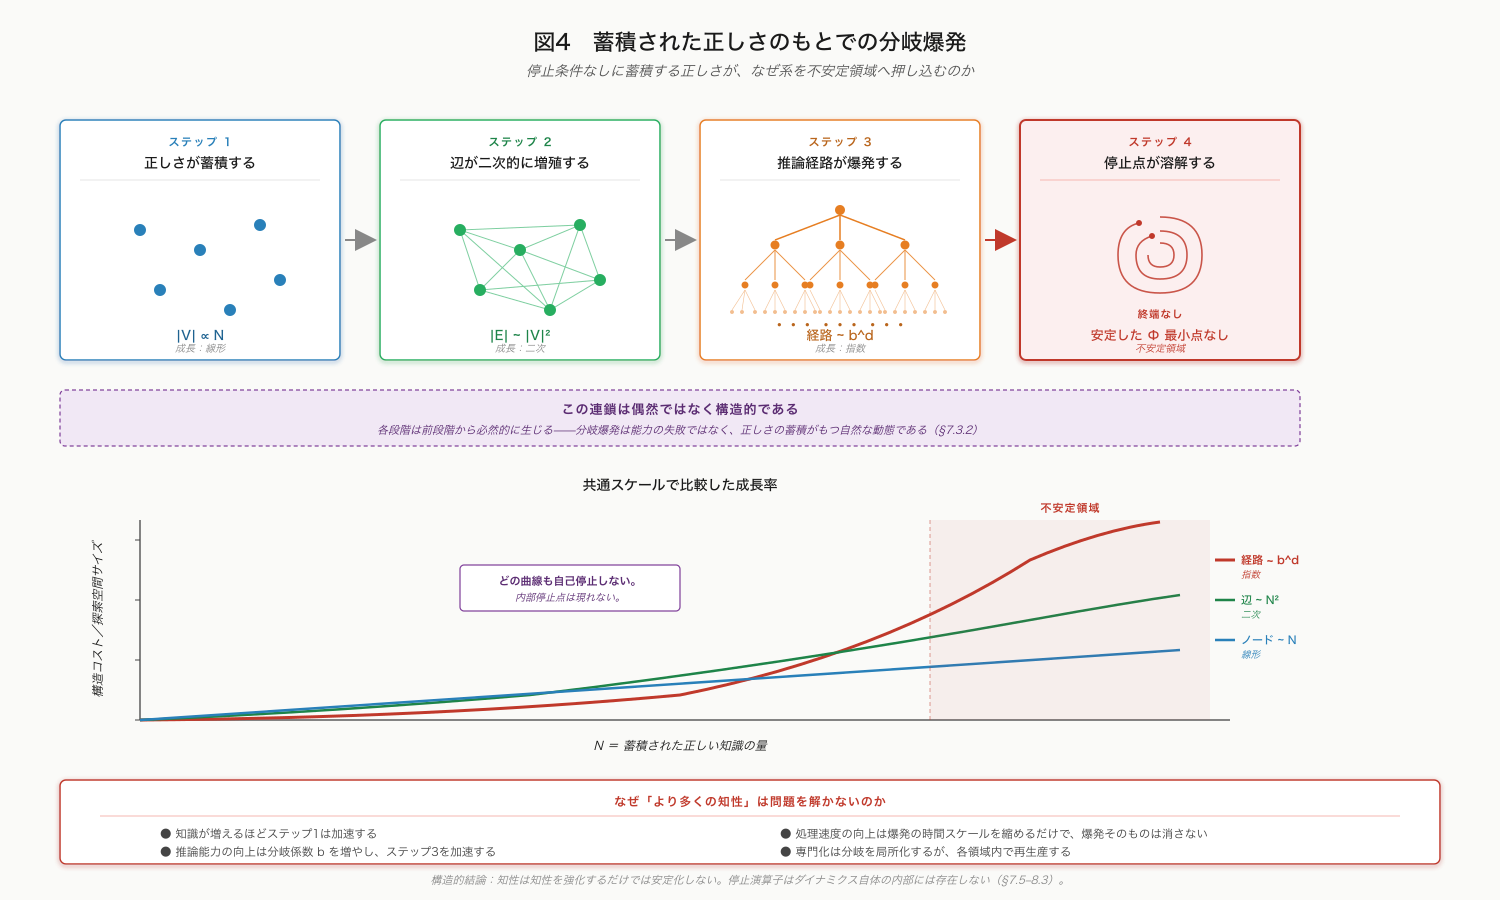
\includegraphics[width=\textwidth]{figures/fig4_branching_explosion_ja.png}
\caption{Branching explosion under accumulated correctness(正しさの累積がノード数線形・エッジ数二次的増大を経て、分岐次数指数的増大に至り、停止点が喪失するまでの動力学的連鎖)}
\label{fig:intelligence_part1_4}
\end{figure}
